\documentclass[../main]{subfiles}

\begin{document}
%%%%%%%%%%%%%%%%%%%%%%%%%%%%%%%%%%%%%%%%%%%%%%%%%%%%%%%%%%%%%%%%%%%%%%%%%
\graphicspath{{images/}}
% To get the right chapter number
\ifSubfilesClassLoaded{
    \externaldocument[main-]{../main}
    \setcounterref{chapter}{main-chap:variabelen-loops}
    \addtocounter{chapter}{-1}
    \setcounter{page}{\getpagerefnumber{main-chap:variabelen-loops}}
}{}
%%%%%%%%%%%%%%%%%%%%%%%%%%%%%%%%%%%%%%%%%%%%%%%%%%%%%%%%%%%%%%%%%%%%%%%%%
\pagestyle{mypagestyle}
\chapterstyle{MyChapterStyle}  

\chapter{Variabelen en loops}
\label{chap:variabelen-loops}

\begin{objectivesbox}
    \begin{objectiveslist}
        \item hoe je met variabelen je code flexibeler maakt;
        \item hoe je met while en for loops code kunt laten herhalen.
    \end{objectiveslist}
\end{objectivesbox}

\begin{wrapfigure}{R}{0.40\textwidth}
    \adjustimage{width=0.9\linewidth, right}{variables_boxes}
\end{wrapfigure}
Waarschijnlijk heb je bij wiskunde of science al eens gehoord van de term \emph{variabele}. In programmeercode is een variabele een naam die verwijst naar een waarde. Een voorbeeld zie je in listing~\ref{lst:variable-example}. Hierin is \texttt{lengte} een variabele met de waarde \texttt{100}. In de aanroep van \texttt{fd()} wordt \texttt{lengte} als argument meegegeven, waardoor de schilpad 100 vooruit gaat.

\vspace{\baselineskip}

\begin{python}[style=mu, caption={De variabele \texttt{lengte}}, label={lst:variable-example}, numbers=none, aboveskip=0.5\baselineskip]
lengte = 100
tony.fd(lengte)
\end{python}

Een variabele wordt soms vergeleken met een doosje waarin je iets kunt bewaren. Het etiket op het doosje staat voor de naam van de variabele, en de inhoud van het doosje staat voor de waarde van de variabele.

\section{Assignment}
\label{sec:assignment}

In Python maak je een variabele aan door een naam te kiezen en die naam een waarde toe te wijzen. Dit proces heet \emph{assignment} (Nederlands: toewijzing).

\begin{figure}[ht]
\centering
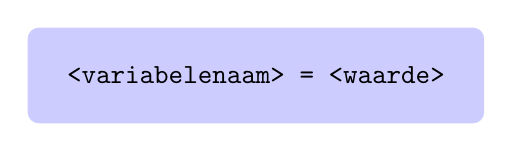
\begin{tikzpicture}
    \node [%
        font=\ttfamily,
        fill=blue!20!white,
        inner sep=5mm,
        rounded corners,]
        {<variabelenaam> = <waarde>};
\end{tikzpicture}
\caption{Assignment in Python}
\label{fig:assignment}
\end{figure}

Je mag de variabelenaam zelf bedenken, maar hij moet wel aan enkele voorwaarden voldoen:
\begin{itemize}
\item De naam moet beginnen met een letter of het underscore karakter (\texttt{\_}).
\item De naam mag niet met een cijfer beginnen.
\item De naam mag alleen letters, cijfers en het underscore karakter bevatten.
\end{itemize}

Variabelenamen zijn hoofdlettergevoelig. Dus \texttt{lengte} en \texttt{Lengte} zijn twee verschillende variabelen. In Python is het gebruikelijk om variabelenamen in kleine letters te schrijven.

In listing~\ref{lst:turtle-variables} zie je op regels 5 en 6 de variabelen \texttt{lengte} en \texttt{breedte} gecreëerd worden. Ook zie je dat de waarde van \texttt{breedte} wordt berekend op basis van de waarde van \texttt{lengte}. Op deze manier kun je variabelen gebruiken om waarden op te slaan en te hergebruiken in je code.

\begin{python}[style=mu, caption={\file{turtle\_variables.py}}, label={lst:turtle-variables}]
import turtle

tony = turtle.Turtle()

lengte = 100
breedte = lengte / 2

tony.fd(lengte)
tony.lt(90)
tony.fd(breedte)
tony.lt(90)
tony.fd(lengte)
tony.lt(90)
tony.fd(breedte)
\end{python}

Kun je bedenken wat het voordeel is van het gebruik van variabelen in listing~\ref{lst:turtle-variables} in vergelijking met het direct gebruiken van getallen in de aanroepen van \texttt{fd()}? Stel je eens voor dat je de rechthoek twee keer zo groot wilt maken. Dan hoef je alleen maar de waarde van \texttt{lengte} aan te passen, en de rest van de code blijft hetzelfde. Zonder variabelen zou je alle getallen in de code moeten aanpassen, wat niet alleen meer werk, maar ook foutgevoelig is.

\begin{infobox}[Datatypes]
Heb je je al afgevraagd of \texttt{tony} in listing~\ref{lst:turtle-variables} ook een variabele is? Dat is inderdaad het geval; regel 3 bevat immers een assignment statement (te herkennen aan het \texttt{=}-teken). Variabelen hoeven niet per se een getal te bevatten, je kunt er ook andere soorten waarden in opslaan, bijvoorbeeld tekst of een lijst. De waarde van \texttt{tony} is een object van het type \texttt{Turtle}.

Het type van een waarde noemen we het \emph{datatype}. In Python kun je het datatype van een waarde opvragen met de functie \texttt{type()}.

\begin{python}[style=mu, numbers=none]
import turtle

tony = turtle.Turtle()

lengte = 100
breedte = lengte / 2

print(type(lengte))
print(type(breedte))
print(type(tony))
\end{python}

De output van deze code zie je hieronder. Gehele getallen hebben in Python het datatype \texttt{int} en kommagetallen (en resultaten van delingen) hebben het datatype \texttt{float}.

\begin{center}
\shellbox[width=10cm]{turtle\_variables.py}{%
<class 'int'>\\
<class 'float'>\\
<class 'turtle.Turtle'>\\
>>>}
\end{center}

\end{infobox}
%%%%%%%%%%%%%%%%%%%%%%%%%%%%%%%%%%%%%%%
\subsection*{Opgaven}

\begin{opgave}[icons={laptop}]
Maak een nieuw codebestand en sla het op als \file{turtle\_triangle.py}. Importeer de \texttt{turtle} module en maak een schildpad aan. Creëer vervolgens een variabele \texttt{size} en geef deze de waarde 100.
\begin{qlist}
\item Laat de schildpad een gelijkzijdige driehoek met zijden van lengte \texttt{size} tekenen.
\item Wijzig je code zodat drie elkaar rakende stippen met diameter \texttt{size} worden getekend in plaats van een driehoek (als in figuur~\ref{fig:turtle-dots-triangle}). Run je code en wijzig daarna de waarde van \texttt{size} (en verder niets!) om te zien wat er gebeurt. Als je het goed hebt gedaan, moeten de stippen elkaar nog steeds raken nadat je de waarde van \texttt{size} hebt aangepast.

\begin{figure}[ht]
    \centering
    \adjustimage{width=0.5\linewidth}{turtle_dots_triangle}
    \caption{Drie elkaar rakende stippen}%
    \label{fig:turtle-dots-triangle}
\end{figure}
\end{qlist}
\end{opgave}
%--------------------------------------
\begin{antwoord}
\begin{qlist}
\item%
\begin{python}[style=mu]
import turtle

tony = turtle.Turtle()

size = 100

tony.fd(size)
tony.lt(120)
tony.fd(size)
tony.lt(120)
tony.fd(size)
\end{python}
\item Hieronder een mogelijke oplossing. Omdat de stippen met de penkleur worden getekend, is het niet nodig de pen omhoog te doen. De getekende lijnen vallen weg tegen de stippen.
\begin{python}[style=mu]
import turtle

tony = turtle.Turtle()

size = 100
tony.dot(size)
tony.fd(size)
tony.lt(120)
tony.dot(size)
tony.fd(size)
tony.lt(120)
tony.dot(size)
\end{python}
\end{qlist}

\end{antwoord}
%%%%%%%%%%%%%%%%%%%%%%%%%%%%%%%%%%%%%%%%%%%
\begin{opgave}[icons={laptop}]
Maak een nieuw codebestand en sla het op als \file{turtle\_target.py}.
\begin{qlist}
\item Schrijf een programma dat een doelwit tekent zoals in figuur~\ref{fig:turtle-target}, en voldoet aan de volgende eisen:
\begin{tasklist}
\item Voor het tekenen van de cirkels mag alleen de \texttt{dot()} functie worden gebruikt.
\item De diameter van de grootste cirkel wordt bepaald door een variabele met de naam \texttt{size}.
\item De diameters van de kleinere cirkels moeten gelijkmatig afnemen. Dus als de grootste cirkel een diameter van 300 heeft, dan moeten de kleinere cirkels diameters van 200 en 100 hebben. Je dient deze diameters te berekenen op basis van de waarde van \texttt{size}, en niet door ze direct in de code te typen.
\end{tasklist}

\begin{figure}[ht]
    \centering
    \adjustimage{width=0.5\linewidth}{turtle_target}
    \caption{Een doelwit}%
    \label{fig:turtle-target}
\end{figure}
\item Wijzig je code zodat een volledig doelwit wordt getekend zoals in figuur~\ref{fig:turtle-target-2}. Voor de buitenste lijn gebruik je de \texttt{circle()} functie. Wanneer je de variabele \texttt{size} aanpast, moeten alle onderdelen van het doelwit evenredig meegroeien of krimpen.

\begin{figure}[ht]
    \centering
    \adjustimage{width=0.5\linewidth}{turtle_target_2}
    \caption{Een volledig doelwit}%
    \label{fig:turtle-target-2}
\end{figure}
\end{qlist}
\end{opgave}
%--------------------------------------
\begin{antwoord}
\begin{qlist}
\item%
\begin{python}[style=mu]
import turtle

tony = turtle.Turtle()

size = 300
tony.dot(size, 'lightskyblue')
tony.dot(size * 2/3, 'red')
tony.dot(size * 1/3, 'yellow')
\end{python}
\item%
\begin{python}[style=mu]
import turtle

tony = turtle.Turtle()

size = 300
tony.dot(size * 4/5, 'black')
tony.dot(size * 3/5, 'lightskyblue')
tony.dot(size * 2/5, 'red')
tony.dot(size * 1/5, 'yellow')
tony.pu()
tony.bk(size / 2)
tony.rt(90)
tony.pd()
tony.circle(size / 2)
\end{python}
\end{qlist}

\end{antwoord}
%%%%%%%%%%%%%%%%%%%%%%%%%%%%%%%%%%%%%%%%%%%
\begin{opgave}[icons={laptop}]
\begin{minipage}[t]{0.6\textwidth}
\raggedright
Maak een nieuw codebestand en sla het op als \file{turtle\_square\_circle.py}.
Schrijf een programma dat een cirkel tekent met daaromheen een vierkant, zoals in figuur~\ref{fig:turtle-square-circle}. De straal van de cirkel wordt bepaald door een variabele met de naam \texttt{radius}. Wanneer je de waarde van \texttt{radius} aanpast, moeten zowel het vierkant als de cirkel evenredig meegroeien of krimpen.
\end{minipage}%
\hfill%
\begin{minipage}[t]{0.3\textwidth}
\adjustimage{width=\linewidth, valign=T, raise=6pt, right}{square_circle}
\captionof{figure}{Een vierkant met een cirkel}%
\label{fig:turtle-square-circle}
\end{minipage}


% \begin{figure}[ht]
%     \centering
%     \adjustimage{width=0.5\linewidth}{turtle_square_circle}
%     \caption{Een vierkant met een cirkel}%
%     \label{fig:turtle-square-circle}
% \end{figure}
\end{opgave}
%--------------------------------------
\begin{antwoord}
\begin{python}[style=mu]
import turtle

tony = turtle.Turtle()

radius = 100
tony.circle(radius)
tony.fd(radius)
tony.lt(90)
tony.fd(2 * radius)
tony.lt(90)
tony.fd(2 * radius)
tony.lt(90)
tony.fd(2 * radius)
tony.lt(90)
tony.fd(radius)
\end{python}
\end{antwoord}
%%%%%%%%%%%%%%%%%%%%%%%%%%%%%%%%%%%%%%%%%%%
\section{While loops}%
\label{sec:while-loops}

Alle code die je tot nu toe hebt geschreven, werd regel voor regel, van boven naar beneden uitgevoerd. Soms wil je echter dat bepaalde instructies meerdere keren worden uitgevoerd. Bijvoorbeeld als je een patroon wilt tekenen dat uit meerdere herhalingen van dezelfde vorm bestaat. Met een \emph{loop} (Nederlands: lus) kun je een blok code meerdere keren laten uitvoeren. In listing~\ref{lst:while-loop} zie je een voorbeeld van een loop die vijf keer de tekst \texttt{Hello, World!} afdrukt.

\begin{python}[style=mu, caption={Een \texttt{while} loop}, label={lst:while-loop}]
teller = 0
while teller < 5:
    print('Hello, World!')
    teller += 1
\end{python}

\begin{center}
\shellbox[width=10cm]{while\_loop.py}{%
Hello, World!\\
Hello, World!\\
Hello, World!\\
Hello, World!\\
Hello, World!}
\captionof{figure}{Output van listing~\ref{lst:while-loop}}%
\label{fig:while-loop-resultaat}
\end{center}

De loop in listing~\ref{lst:while-loop} is een zogenoemde \texttt{while} loop, te herkennen aan het keyword \texttt{while} in regel 2. Je zou \emph{while} naar het Nederlands kunnen vertalen als \emph{zolang}. Op regel 2 staat dus eigenlijk: Zolang de waarde van \texttt{teller} kleiner is dan 5, blijf dan het volgende blok code uitvoeren. Het blok code dat herhaald wordt, is in dit geval regel 3 en regel 4. Je kunt zien dat deze regels ingesprongen zijn ten opzichte van regel 2. Dat is belangrijk. Daardoor weet Python dat regels 3 en 4 zich binnen de \texttt{while} loop bevinden. 
Regel 4 bevat de opdracht \texttt{teller += 1}. Dit is een verkorte notatie voor \texttt{teller = teller + 1}. In deze regel wordt de waarde van \texttt{teller} dus met 1 verhoogd. Daardoor stopt de loop na vijf keer. Zonder regel 4 zou de waarde van \texttt{teller} altijd \texttt{0} blijven, en zou de loop oneindig doorgaan.

\clearpage
Figuur~\ref{fig:flowchart-while} toont het stroomdiagram van een \texttt{while} loop. Je ziet dat na het uitvoeren van het codeblok wordt teruggesprongen naar de voorwaarde. De voorwaarde wordt opnieuw geëvalueerd, en als deze nog steeds \texttt{True} is, wordt het codeblok weer uitgevoerd. 

\begin{figure}[ht]
\centering
\scalebox{0.8}{
    \begin{tikzpicture}[
        node distance=1cm,
        every node/.style={%
            font=\sffamily
        },
        box/.style={%
            draw=green!40!black,
            font=\sffamily\large,
            text centered,
            thick,
        },
        startstop/.style={%
            box,
            rectangle,
            rounded corners=5mm,
            minimum width=2cm,
            minimum height=1cm,
            fill=green!10!white,
        },
        process/.style={%
            box,
            rectangle,
            minimum width=3cm,
            minimum height=1cm,
            fill=green!3!white,
            inner sep=5pt,
        },
        decision/.style={%
            box,
            diamond,
            aspect=2,
            text width=3cm,
            inner sep=0pt,
            fill=green!3!white,
        },
        arrow/.style={%
            -{Stealth[width=2mm]},
            thick,
            draw=green!40!black,
        }
        ]
        \node (start) at (2,8) [startstop] {Start};
        \node (voorwaarde) [decision, below=of start] {Voorwaarde?};
        \node (actietrue) [process, below=1.5cm of voorwaarde, align=center] {Code block};
        \node (stop) [startstop, below=1cm of actietrue] {Stop};
        \node (false) [right=0mm of voorwaarde, yshift=3mm] {False};
        \path (start) edge[arrow] (voorwaarde)
            (voorwaarde.south) edge[arrow] node[auto, swap, yshift=3mm] {True} (actietrue.north)
            (voorwaarde.east) edge[arrow, to path={-- ++(1cm,0) |- (\tikztotarget)}] (stop.east)
            (actietrue.west) edge[arrow, to path={-- ([xshift=-1cm]actietrue.west) |- (voorwaarde.west)}] (voorwaarde.west);
    \end{tikzpicture}}
    \caption{Flowchart while loop}%
    \label{fig:flowchart-while}
\end{figure}

Voor de voorwaarde in een \texttt{while} loop kun je elke uitdrukking gebruiken die resulteert in een \texttt{True} of \texttt{False} waarde. In listing~\ref{lst:while-loop} is dat de vergelijking \texttt{teller < 5}. Tabel \ref{tbl:vergelijkingsoperatoren} geeft een overzicht van de vergelijkingsoperatoren die je kunt gebruiken in een voorwaarde.

\begin{table}[ht]
    \centering
    \begin{tblr}{
       colspec={Q[c]Q[l]Q[c]Q[c]},
        column{1,3,4} = {font=\ttfamily},
        column{3} = {leftsep=1cm},
        row{1} = {font=\sffamily\bfseries},
        stretch=1.5}
        \topline
        Operator & Naam & Voorbeeld & Uitkomst \\
        \clinels{1}\clinems{2,3}\cliners{4}
        == & Gelijk aan  & 1 == 2    & False \\
        != & Ongelijk aan & 1 != 2    & True \\
        <  & Kleiner dan & 4 < 5     & True \\
        >  & Groter dan  & 3 > 3     & False \\
        <= & Kleiner of gelijk aan & 4 <= 5 & True \\
        >= & Groter of gelijk aan & 3 >= 3 & True \\
        \bottomline
    \end{tblr}
    \caption{Vergelijkingsoperatoren in Python.}%
    \label{tbl:vergelijkingsoperatoren}
\end{table}

Wanneer je tijdens het programmeren merkt dat je telkens dezelfde regels aan het typen (of aan het kopiëren en plakken) bent, moet je jezelf afvragen of je misschien een loop kunt gebruiken. Je code wordt er namelijk korter door en daarmee eleganter, makkelijker te begrijpen en minder foutgevoelig. In listing~\ref{lst:turtle-vierkant} en listing~\ref{lst:turtle-vierkant-while} zie je dat in praktijk gebracht voor het tekenen van een vierkant.
De code in listing~\ref{lst:turtle-vierkant-while} is korter, en bovendien is duidelijker dat er vier keer dezelfde acties worden uitgevoerd, namelijk vooruit gaan en linksaf slaan.

\noindent\begin{minipage}[t]{.45\textwidth}
\begin{python}[style=mu, caption={Vierkant op de oude manier}, label={lst:turtle-vierkant}]
import turtle

tony = turtle.Turtle()

tony.fd(100)
tony.lt(90)
tony.fd(100)
tony.lt(90)
tony.fd(100)
tony.lt(90)
tony.fd(100)
\end{python}
\end{minipage}\hfill
\begin{minipage}[t]{.45\textwidth}
\begin{python}[style=mu, caption={Vierkant met while loop}, label={lst:turtle-vierkant-while}]
import turtle

tony = turtle.Turtle()

zijde = 0
while zijde < 4:
    tony.fd(100)
    tony.lt(90)
    zijde += 1
\end{python}
\end{minipage}

Het voordeel van loops wordt nóg duidelijker als je een patroon wilt tekenen dat uit meerdere herhalingen van dezelfde vorm bestaat. In listing~\ref{lst:nested-code-blocks} zie je een voorbeeld van een patroon dat bestaat uit acht vierkanten naast elkaar. De code maakt gebruik van \emph{geneste} \texttt{while} loops. De buitenste \texttt{while} loop zorgt ervoor dat het vierkant acht keer wordt getekend, en de binnenste \texttt{while} loop zorgt ervoor dat elk vierkant uit vier zijden bestaat.\\
Zonder gebruikmaking van loops zou je voor het tekenen van dezelfde acht vierkanten maar liefst 87 regels code nodig hebben, terwijl je mét loops aan slechts 13 regels genoeg hebt. Dat is een enorm verschil!

\begin{figure}[ht]
    \centering
    \adjustimage{width=0.5\linewidth}{turtle_squares}
    \caption{Output van listing~\ref{lst:nested-code-blocks}}%
    \label{fig:turtle-squares}
\end{figure}

\begin{python}[style=mu, caption={Geneste \texttt{if} statements}, label={lst:nested-code-blocks},name=nestedcodeblocks, framextopmargin=3pt, framexleftmargin=3pt, lineskip=3pt,]
import turtle

tony = turtle.Turtle()

vierkant = 0
while vierkant < 8:
    zijde = 0
    while zijde < 4:
        tony.fd(40)
        tony.lt(90)
        zijde += 1
    tony.pu()
    tony.fd(50)
    tony.pd()
    vierkant += 1
\end{python}

\begin{tikzpicture}[overlay, remember picture]
     \xdef\boundingboxblocka{%
    (pic cs:line-nestedcodeblocks-0-start)%
    ([xshift=\linewidth-3pt]pic cs:line-nestedcodeblocks-0-start)%
    ([yshift=-2pt]pic cs:line-nestedcodeblocks-15-start)}
    \xdef\boundingboxblockb{%
    (pic cs:line-nestedcodeblocks-7-first)%
    ([xshift=\linewidth-15pt, yshift=8pt]pic cs:line-nestedcodeblocks-7-start)%
    ([yshift=-2pt]pic cs:line-nestedcodeblocks-15-first)}
    \xdef\boundingboxblockc{%
    (pic cs:line-nestedcodeblocks-9-first)%
    ([xshift=\linewidth-30pt, yshift=8pt]pic cs:line-nestedcodeblocks-9-start)%
    ([yshift=-1pt]pic cs:line-nestedcodeblocks-11-first)}
    \node[%
        draw=red,
        line width=2pt,
        rounded corners=2pt,
        dotted,
        fit=\boundingboxblocka,
        ] (block1) {};
    \node[%
        align=right,
        draw=blue,
        line width=2pt,
        rounded corners=2pt,
        dotted,
        fit=\boundingboxblockb,
        ] (block2) {};
    \node[%
        align=right,
        draw=green!60!black,
        line width=2pt,
        rounded corners=2pt,
        dotted,
        fit=\boundingboxblockc,
        ] (block3) {};
    \node[%
        anchor=north east,
        text=red,
        font=\sffamily\bfseries\Large,
    ] at ([shift={(-2pt,-2pt)}]block1.north east) {Block 1};
    \node[%
        anchor=north east,
        text=blue,
        font=\sffamily\bfseries\Large,
    ] at ([shift={(-2pt,-2pt)}]block2.north east) {Block 2};
    \node[%
        anchor=north east,
        text=green!60!black,
        font=\sffamily\bfseries\Large,
    ] at ([shift={(-2pt,-2pt)}]block3.north east) {Block 3};
\end{tikzpicture} 

Zoals gezegd moet je bij loops goed letten op de inspringing van coderegels. Om duidelijk te maken welke code bij welke loop hoort, zijn de codeblokken in listing~\ref{lst:nested-code-blocks} met verschillende kleuren omkaderd. De regels 9, 10 en 11 zijn twee keer ingesprongen, terwijl bijvoorbeeld regel 12 slechts eenmaal ingesprongen is. Regel 12 valt dus binnen de buitenste \texttt{while} loop, maar buiten de binnenste \texttt{while} loop.

\begin{infobox}[De Tab toets]
In Python is het belangrijk dat de inspringing van coderegels consistent is. Dat betekent dat je niet zomaar een willekeurig aantal spaties kunt gebruiken om regels in te springen. Je moet altijd hetzelfde aantal spaties gebruiken voor regels die zich op hetzelfde niveau van inspringing bevinden, anders krijg je een foutmelding.

Om dit makkelijker te maken, kun je het beste de \keys{Tab} toets gebruiken om regels in te springen (en dus niet de spatiebalk!). De \keys{Tab} toets bevindt zich meestal links op je toetsenbord, boven de \keys{Caps Lock} toets. 
\end{infobox}
%%%%%%%%%%%%%%%%%%%%%%%%%%%%%%%%%%%%%%%
\subsection*{Opgaven}

\begin{opgave}[icons={laptop}]
Maak een nieuw codebestand en sla het op als \file{turtle\_triangle\_loops.py}. Importeer de \texttt{turtle} module en maak een schildpad aan. 
\begin{qlist}
\item Schrijf een programma dat met behulp van een \texttt{while} loop een gelijkzijdige driehoek tekent met zijden van 100. Na het tekenen van een zijde moet de schilpad telkens 120\textdegree{} draaien. Als je er niet uitkomt, kijk dan nog eens naar listing~\ref{lst:turtle-vierkant-while}.
\item Maak een tweede while loop en plaats een deel van de code van onderdeel \textsf{a} daarin (door de regels in te springen). Zorg ervoor dat er vier driehoeken naast elkaar worden getekend, zoals in figuur~\ref{fig:turtle-triangles}. Voor inspiratie kun je kijken naar listing~\ref{lst:nested-code-blocks}.

\begin{figure}[ht]
    \centering
    \adjustimage{width=0.5\linewidth}{triangles_in_a_row}
    \caption{Vier driehoeken naast elkaar}%
    \label{fig:turtle-triangles}
\end{figure}
\end{qlist}
\end{opgave}
%--------------------------------------
\begin{antwoord}
\begin{qlist}
\item%
\begin{python}[style=mu]
import turtle

tony = turtle.Turtle()

zijde = 0
while zijde < 3:
    tony.fd(100)
    tony.lt(120)
    zijde = zijde + 1
\end{python}
\item Hieronder een mogelijke oplossing. Omdat de stippen met de penkleur worden getekend, is het niet nodig de pen omhoog te doen. De getekende lijnen vallen weg tegen de stippen.
\begin{python}[style=mu]
import turtle

tony = turtle.Turtle()

driehoek = 0
while driehoek < 4:
    zijde = 0
    while zijde < 3:
        tony.fd(100)
        tony.lt(120)
        zijde = zijde + 1
    tony.fd(100)
    driehoek = driehoek + 1
\end{python}
\end{qlist}

\end{antwoord}
%%%%%%%%%%%%%%%%%%%%%%%%%%%%%%%%%%%%%%%%%%%
\begin{opgave}[icons={laptop}]
Maak een nieuw codebestand en sla het op als \file{turtle\_square\_star.py}. Schrijf een programma dat met behulp van geneste \texttt{while} loops een `ster' tekent bestaande uit 20 vierkanten, waarbij elk vierkant 18\textdegree{} gedraaid is ten opzichte van het vorige vierkant, zoals in figuur~\ref{fig:turtle-squares-star}. De zijden van de vierkanten hebben lengte 100.

\begin{figure}[ht]
    \centering
    \adjustimage{width=0.3\linewidth}{flower_of_squares}
    \caption{Een ster van vierkanten}%
    \label{fig:turtle-squares-star}
\end{figure}
\end{opgave}
%--------------------------------------
\begin{antwoord}
\begin{python}[style=mu]
import turtle

tony = turtle.Turtle()

vierkant = 0
while vierkant < 20:
    zijde = 0
    while zijde < 4:
        tony.fd(100)
        tony.lt(90)
        zijde += 1
    tony.lt(18)
    vierkant += 1
\end{python}
\end{antwoord}
%%%%%%%%%%%%%%%%%%%%%%%%%%%%%%%%%%%%%%%%%%%
\begin{opgave}[icons={laptop}]
Maak een nieuw codebestand en sla het op als \file{turtle\_dot\_pattern.py}. Neem onderstaande code over in je bestand en vervang de puntjes door code die ervoor zorgt dat een rooster van 10 bij 10 rode stippen wordt getekend, zoals in figuur~\ref{fig:turtle-dot-pattern}. Merk op dat in regel 6 de pen van het papier wordt gehaald, want voor het tekenen van dots is het niet nodig dat de pen op het papier staat. De pen kan dus gedurende het gehele programma omhoog blijven.

\begin{python}[style=mu, caption={Basiscode voor een stippenpatroon}, label={lst:turtle-dot-pattern}]
import turtle

tony = turtle.Turtle()
tony.hideturtle()
tony.speed(0)
tony.pu()

rij = 0
while ...:
    kolom = 0
    while ...:
        tony.dot(20, 'red')
        ...
        ...
        ...
    ...
    ...
    ...
    ...
    ...
\end{python}

\begin{figure}[ht]
    \centering
    \adjustimage{width=0.3\linewidth}{red_dots}
    \caption{Een stippenpatroon}%
    \label{fig:turtle-dot-pattern}
\end{figure}
\end{opgave}
%--------------------------------------
\begin{antwoord}
\begin{python}[style=mu]
import turtle

tony = turtle.Turtle()
tony.hideturtle()
tony.speed(0)
tony.pu()

rij = 0
while rij < 10:
    kolom = 0
    while kolom < 10:
        tony.dot(20, 'red')
        tony.fd(30)
        kolom += 1
    tony.bk(300)
    tony.lt(90)
    tony.fd(30)
    tony.rt(90)
    rij += 1
\end{python}
\end{antwoord}
%%%%%%%%%%%%%%%%%%%%%%%%%%%%%%%%%%%%%%%%%%%
\begin{opgave}[icons={laptop}]
Het wordt nóg interessanter wanneer je de \texttt{while} loop variabele niet alleen als teller gebruikt, maar bijvoorbeeld ook als argument aan de functie \texttt{fd()} meegeeft. Neem de code uit listing~\ref{lst:turtle-spiral} over in een nieuw bestand \file{turtle\_spiral.py}. Je ziet dat in regel 7 de variabele \texttt{lengte} als argument aan \texttt{tony.fd()} wordt meegegeven. Deze variabele wordt in regel 9 telkens met 2 opgehoogd. Daardoor legt onze schildpad dus steeds grotere afstanden af.

\begin{python}[style=mu, caption={Spiraal}, label={lst:turtle-spiral}]
import turtle

tony = turtle.Turtle()

lengte = 2
while lengte < 300:
    tony.fd(lengte)
    tony.lt(30)
    lengte = lengte + 2
\end{python}

Run de code en experimenteer ermee door telkens één getal een beetje te veranderen en te bekijken hoe de figuur verandert. En wat gebeurt er als je op regel 8 \texttt{tony.lt(30)} vervangt door \texttt{tony.lt(lengte)} of door \texttt{tony.lt(3 * lengte)}? Probeer maar uit!
\end{opgave}
%--------------------------------------
\begin{antwoord}
*
\end{antwoord}

\begin{figure}[h]
    \adjustimage{width=0.6\linewidth, center}{loopings}
\end{figure}
%%%%%%%%%%%%%%%%%%%%%%%%%%%%%%%%%%%%%%%%%%%
\section{For loops}%
\label{sec:for-loops}

Wanneer je van tevoren al weet hoe vaak je een blok code wilt herhalen, is een while loop enigszins omslachtig. Je hebt er namelijk drie regels code voor nodig (figuur~\ref{lst:while-loop-structure}):
\begin{itemize}[topsep=2pt, itemsep=2pt, parsep=0pt]
\item één om de teller variabele te maken met een assignment statement;
\item één waarin het keyword while staat, gevolgd door de voorwaarde(n);
\item één waarin de waarde van de teller variabele wordt bijgewerkt.
\end{itemize}
Met een \texttt{for} loop kun je hetzelfde bereiken met slechts één regel code (figuur~\ref{lst:for-loop-structure}).

\noindent\begin{minipage}[t]{.45\textwidth}
\begin{python}[style=mu, caption={Een standaard while loop}, label={lst:while-loop-structure}]
n = 0
while n < 10:
    ...
    ...
    n += 1
\end{python}
\end{minipage}\hfill
\begin{minipage}[t]{.45\textwidth}
\begin{python}[style=mu, caption={Een for loop}, label={lst:for-loop-structure}]
for n in range(10):
    ...
    ...
\end{python}
\end{minipage}

% \begin{python}[style=mu, caption={Een standaard while loop}, label={lst:while-loop-standaard}]
% n = 0
% while n < 10:
%     ...
%     ...
%     n += 1
% \end{python}

% Met een \texttt{for} loop kun je hetzelfde bereiken met slechts één regel code.

% \begin{python}[style=mu, caption={Een for loop}, label={lst:for-loop}, aboveskip=2pt]
% for n in range(10):
%     ...
%     ...
% \end{python}

De functie \texttt{range(\textit{stop})} genereert een reeks van gehele getallen van 0 tot en met \texttt{\textit{stop}-1}. In listing~\ref{lst:for-loop-structure} genereert \texttt{range(10)} dus de getallen 0, 1, 2, 3, 4, 5, 6, 7, 8 en 9. De for loop zorgt ervoor dat het codeblok onder regel 1 tien keer wordt uitgevoerd, waarbij de variabele \texttt{n} achtereenvolgens de waarden van deze reeks aanneemt.

Met \texttt{for} loops kun je de code van listing~\ref{lst:nested-code-blocks} herschrijven, zodat je de code in listing~\ref{lst:nested-code-blocks-for} krijgt. De eerste regels zijn weliswaar weggelaten, maar de code voor het tekenwerk is ook daadwerkelijk korter geworden. Bovendien is nog duidelijker dat het codeblok in de buitenste loop acht keer wordt uitgevoerd, en het codeblok in de binnenste loop vier keer.

\begin{python}[style=mu, caption={De while loops uit listing~\ref{lst:nested-code-blocks} vervangen door for loops}, label={lst:nested-code-blocks-for}, firstnumber=5]
for vierkant in range(8):
    for zijde in range(4):
        tony.fd(40)
        tony.lt(90)
    tony.pu()
    tony.fd(50)
    tony.pd()
\end{python}
%%%%%%%%%%%%%%%%%%%%%%%%%%%%%%%%%%%%%%%%%%%
\clearpage
\begin{opgave}[icons={laptop}]
Maak nieuwe codebestand en sla het op als \file{turtle\_star.py}. Schrijf een programma dat een vijfpuntige ster tekent zoals in figuur~\ref{fig:turtle-star}. Je mag zelf de kleur en de pendikte bepalen, maar voor het daadwerkelijke tekenen mag je maximaal 3 regels code gebruiken.

\begin{figure}[ht]
    \centering
    \adjustimage{width=0.3\linewidth}{five_pointed_star}
    \caption{Een vijfpuntige ster}%
    \label{fig:turtle-star}
\end{figure}

\begin{hints}
\item Vind je het lastig om de draaiingshoek te bepalen? Bedenk dan dat de turtle tijdens het tekenen van de ster in totaal 2 keer volledig ronddraait (dus de totale draaiingshoek is \(2 \times 360\unit{\degree} = 720\unit{\degree}\)) en dat die volledige draai over 5 stappen wordt verdeeld.
\end{hints}
\end{opgave}
%--------------------------------------
\begin{antwoord}
\begin{python}[style=mu, numbers=none]
for n in range(5):
    tony.fd(200)
    tony.rt(144)
\end{python}
\end{antwoord}
%%%%%%%%%%%%%%%%%%%%%%%%%%%%%%%%%%%%%%%%%%%
\begin{opgave}[icons={laptop}]
Maak nieuwe codebestand en sla het op als \file{turtle\_square\_flower.py}. Schrijf een programma dat de `bloem' tekent zoals getoond in figuur~\ref{fig:turtle-squares-flower}. De bloem bestaat uit 10 vierkanten met zijden van lengte 100. Om hem te tekenen heb je twee \texttt{for} loops nodig: één om iets 10 keer uit te voeren en daarbinnen één om een vierkant te tekenen.

\begin{subfigures}
    \begin{figure}[ht]
        \begin{minipage}[c]{0.45\linewidth}
                \adjustimage{width=0.8\linewidth, center}{flower_of_squares_2}
                \caption{Bloem van vierkanten}
                \label{fig:turtle-squares-flower}
        \end{minipage}
        \hfill
        \begin{minipage}[c]{0.45\linewidth}
                \adjustimage{width=0.8\linewidth, center}{flower_of_squares_3}
                \caption{Verder verfraaid}
                \label{fig:turtle-squares-flower-2}
        \end{minipage}
    \end{figure}
\end{subfigures}

Je kunt de bloem nog mooier maken door \texttt{fillcolor()}, \texttt{begin\_fill()} en \texttt{end\_fill()} te gebruiken en een stip in het midden te plaatsen (figuur~\ref{fig:turtle-squares-flower-2}).
\end{opgave}
%--------------------------------------
\begin{antwoord}
\begin{python}[style=mu, numbers=none]
import turtle

tony = turtle.Turtle()
tony.pencolor('purple')
tony.fillcolor('skyblue')
tony.pensize(3)
tony.hideturtle()
tony.speed(0)

tony.begin_fill()
for vierkant in range(10):
    for zijde in range(4):
        tony.fd(100)
        tony.lt(90)
    tony.lt(36)
tony.end_fill()
tony.dot(60, 'yellow')
\end{python}
\end{antwoord}
%%%%%%%%%%%%%%%%%%%%%%%%%%%%%%%%%%%%%%%%%%%

% \clearpage
% \pagestyle{empty}
% \section*{Antwoorden hoofdstuk 3}
% \printsolutions[headings=false]

\end{document}
